
\section{Events and Triggers}

In this part the concepts and ideas of both events and triggers will
be explained. We will go through their intention and how to use them
with the engine. Furthermore, a couple of examples will be provided
to give the general idea of what they can be used for. 


\subsection{Concept}

In the natural world, all actions have a reaction, these reactions
could be thought of as events meant to trigger when such actions are
performed. Thus an engine for modeling a virtual environment must
provide as many features as those of the real world environment.


\paragraph*{Events}

To be clear, an event in the context of this engine is the occurrence
of something, for instance an event could be that \textquotedblleft{}an
Agent has moved\textquotedblright{}, or \textquotedblleft{}an Agent
has picked up an item\textquotedblright{}. Furthermore, an event also
has the duty of providing necessary information for the listener,
giving the listener a correct idea of the meaning behind an event.
In the case of the event which signified the movement of an agent,
it is necessary to provide the listener %
\footnote{Listeners refer to the object which is listening to the occurrence
of an event, with the intent of reacting to it%
} with information of which direction the agent moved, where its starting
position is and how far it has moved. Since a listener might be operating
in a different thread, the listener is completely dependent on this
information, as it might no longer be retrievable at the time the
event is being analyzed. For instance, if an agent moved and then
was killed and removed from the world, its position would no longer
be stored in the world. As such, the listener would have no way to
determine where the move had ended if this information was not provided
in the event.


\paragraph*{Triggers}

Triggers in our engine are the means to which listeners gain access
to events. A trigger in our engine is the combination of three different
parts.
\begin{itemize}
\item Events
\item Condition
\item Action\end{itemize}
\begin{description}
\item [{The~events}] are what the trigger is listening for. These can
be any type of event, and a trigger can be registered to any number
of events. But only one event is required to \textquotedblleft{}trigger\textquotedblright{}
a Trigger. For instance, if a Trigger is listening on both the events
\textquotedblleft{}10 seconds passed\textquotedblright{} and \textquotedblleft{}Agent
has moved\textquotedblright{}, then the Trigger will be \textquotedblleft{}triggered\textquotedblright{}
when either of these events occur. However it will be triggered each
and every time such event has occurred and is not limited to just
one occurrence.
\item [{The~Condition}] is a built in predicate for the trigger to check
if it is willing to respond to the event. If the condition is satisfied,
the trigger\textquoteright{}s action is fired. A condition should
only be used in cases that is not covered by another event. For instance,
say you have the event \textquotedblleft{}An agent has moved\textquotedblright{}.
Let us call the agent that moved $a_{m}$ and the agent whose movement
you are interested in $a_{i}$. The condition on the trigger would
then be: 
\[
\textrm{\textbf{is }}a_{m}=a_{i}\textbf{ ?}
\]
\\
As we can see the condition narrows the range of events that are responded
to at the cost of added calculations. In this case it would be much
better to subscribe to the event \textquotedblleft{}Agent $a_{i}$
has moved\textquotedblright{}. This is purely an example as events
can not be tied to specific entity instantiations as events are defined
at compile time.
\item [{The~Action}] of a trigger is the part that performs the work,
it is a method which is executed once an event has been raised and
the condition is satisfied. For instance if a trigger is meant to
write a message when a specific event has occurred, then this is where
the action of writing such a message should be placed.
\end{description}

\subsection{Entities and \texttt{EventManager}}

For triggers to become part of the engine it is required that the
trigger is registered to the engine, however it is of crucial importance
what one registers the trigger to. A trigger can be registered to
either a specific entity or the \texttt{EventManager}. A Trigger registered
to the \texttt{EventManager} will be triggered each time an \texttt{Event}
that it is listening to is fired. However a \texttt{Trigger} registered
to a specific entity will only be informed of events raised on the
specific entity instead of when the event is raised for every single
entity. 

An example of this would be: assume you have a Trigger \texttt{$\mathtt{T_{1}}$}
with the event \textquotedblleft{}An agent has moved\textquotedblright{},
and \texttt{$\mathtt{T_{1}}$} is registered to Agent \texttt{A}.
Additionally, you have a Trigger \texttt{$\mathtt{T_{2}}$} with same
event as \texttt{$\mathtt{T_{1}}$,} but this trigger is registered
to the EventManager. To give a complete picture, also assume there
is an Agent \texttt{B} which has no Triggers registered to it.

This provides us with two scenarios:
\begin{description}
\item [{Agent~\texttt{A}~has~moved:}] In this case, both \texttt{$\mathtt{T_{1}}$}
and \texttt{$\mathtt{T_{2}}$} is triggered, since \texttt{$\mathtt{T_{1}}$}
listens on Agent \texttt{A} and \texttt{$\mathtt{T_{2}}$} listens
on any\texttt{ }agent moving.
\item [{Agent~\texttt{B}~has~moved:}] In this case, only $\mathtt{T_{2}}$
is triggered, for the reasons stated above.
\end{description}

\subsection{Example of making and using an \texttt{Event}}

Let\textquoteright{}s assume one was to make an event which was fired
each time an agent had moved, let us name this Event: \texttt{AgentMoved}.

First, make a class extending the \texttt{XmasEvent} class as shown
below:

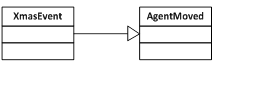
\includegraphics{XmasEventCreationStepOne}

Then, add all the necessary data fields on the newly created event
class.

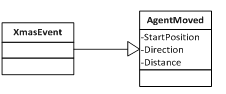
\includegraphics{XmasEventCreationStepTwo}

To utilize the newly created event, it must be raised when appropriate.
In this case, the appropriate place would be to raise it during a
move action.

In this action, after the movement of the agent had been performed,
the method \texttt{RaiseEvent} would need to be called on the entity
that is being moved.


\subsection*{Summary}

Events are what provides the engine flexibility and allows making
reactions to others actions. Events are designed for ease of use and
are meant to be used as much as possible. Triggers are used as a way
to interface with events and they are the only way to connect an object
to the event it wishes to listen to.
